\section{Question 2}
\subsection{1(a)}
\texttt{MDP.py}
\begin{lstlisting}[numbers=none]
J_opt[t,s_index] = min([stage_cost_c(s_index, a) + sum([transition_prob[a, s_index, s_next] * J_opt[t + 1, s_next] for s_next in range(S)]) for a in range(A)])
\end{lstlisting}

\subsection{1(b)}
\begin{figure}[H]
\centering
\begin{subfigure}{0.49\textwidth}
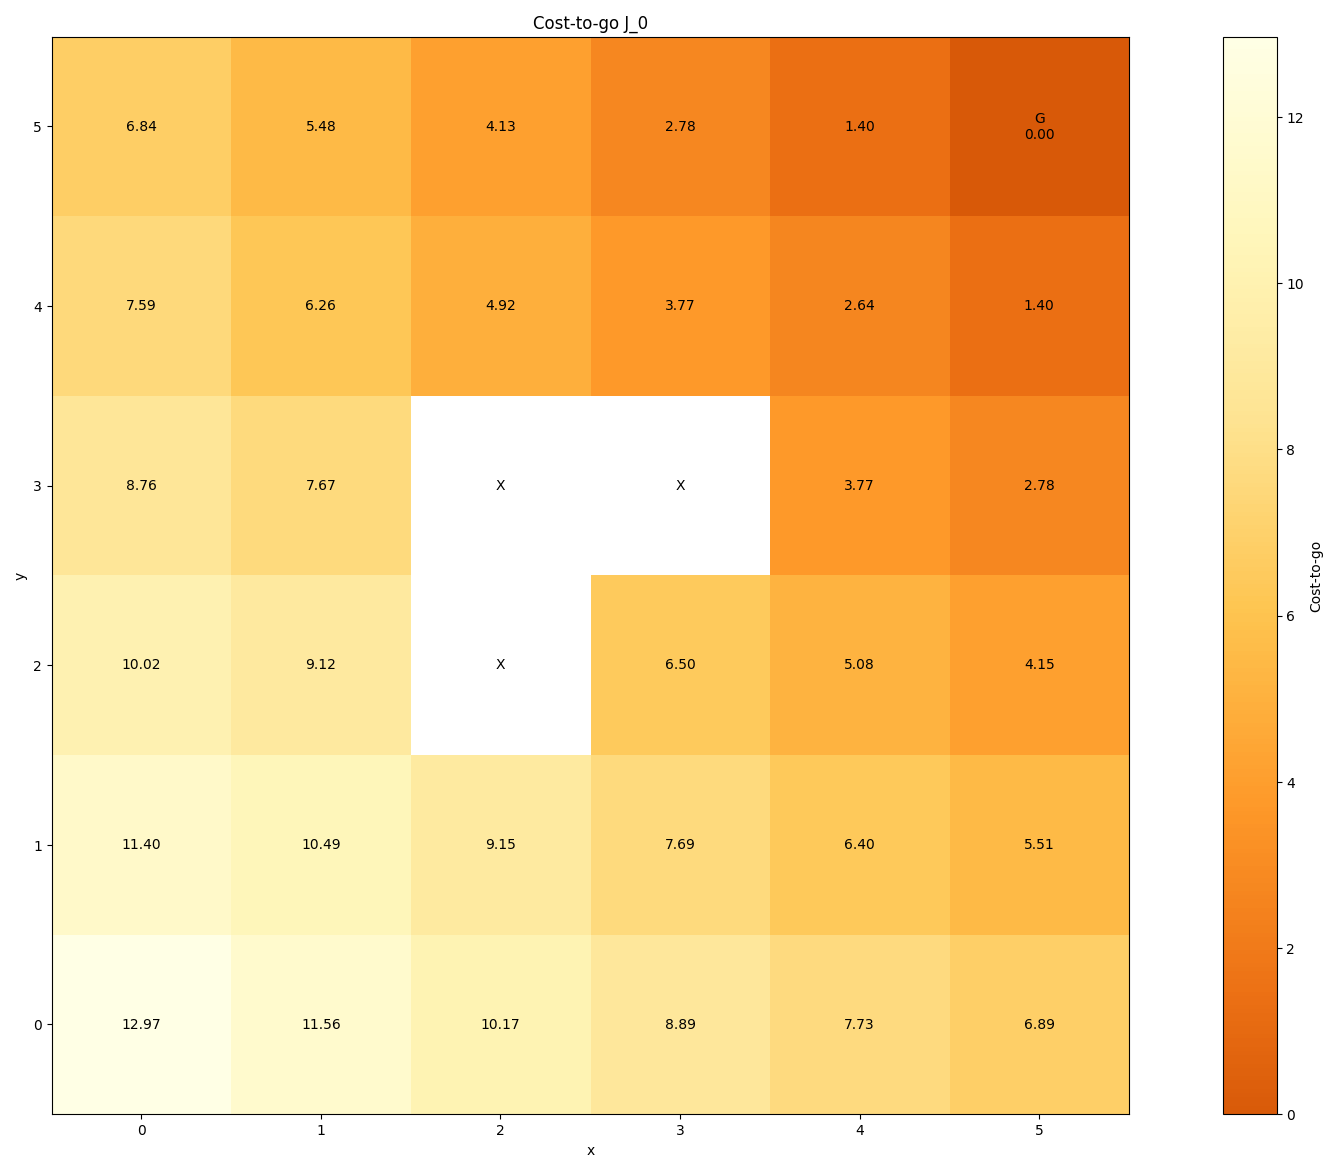
\includegraphics[width=\textwidth]{report_figures/j0_part1.png}
\caption{$J_0^*$}
\end{subfigure}\hfill
\begin{subfigure}{0.49\textwidth}
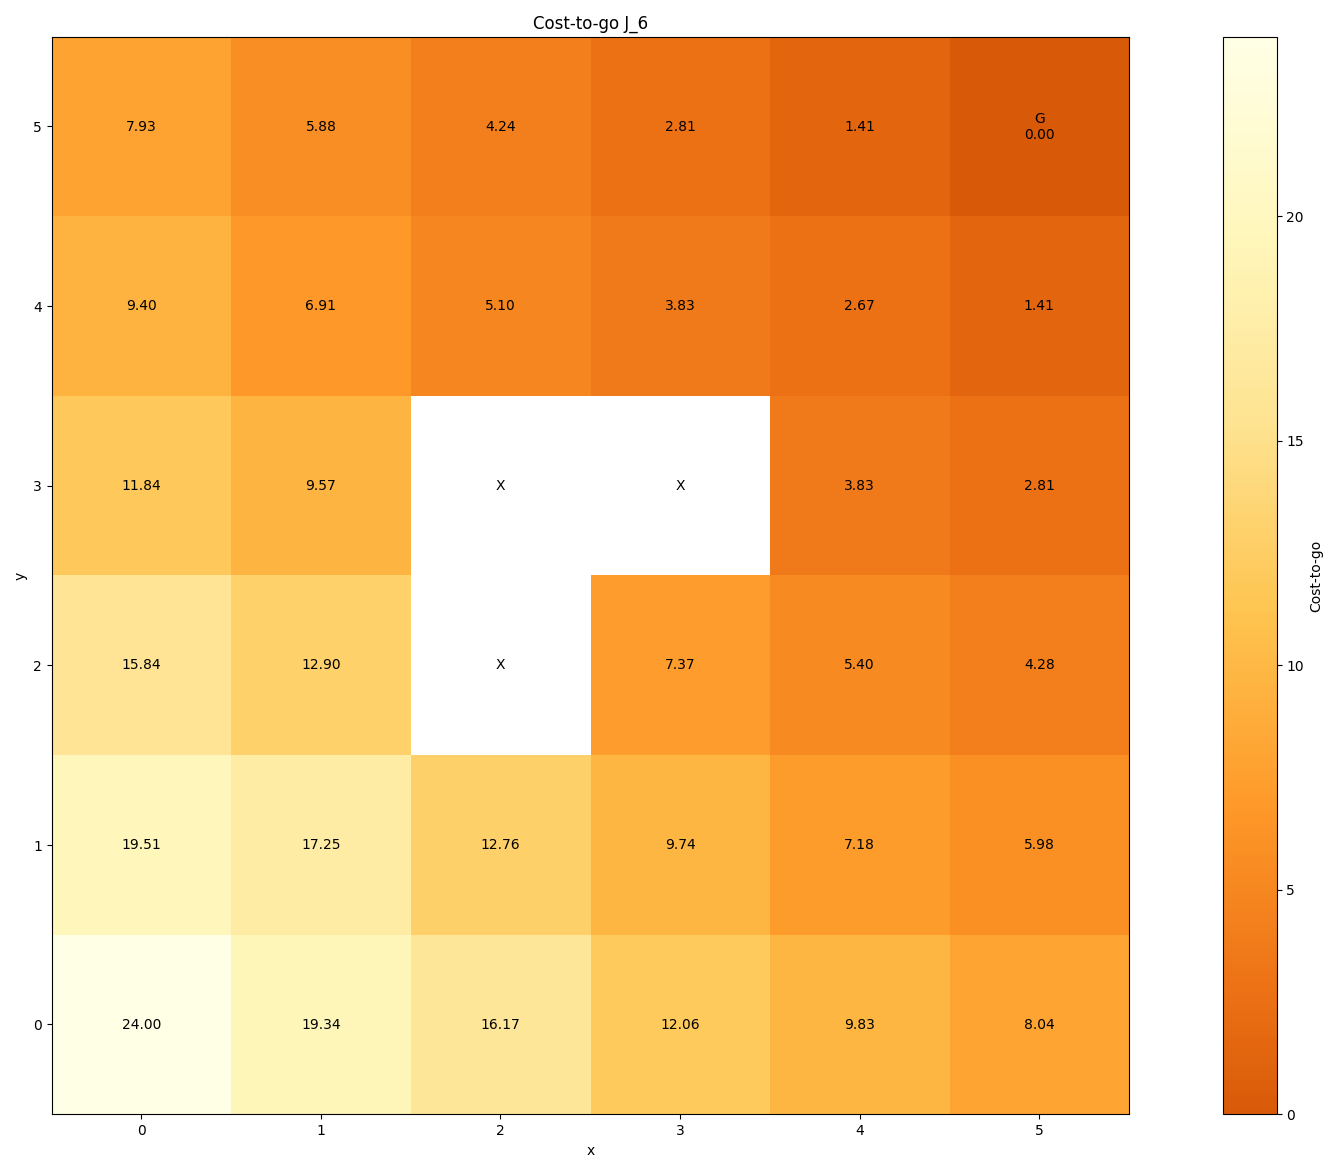
\includegraphics[width=\textwidth]{report_figures/j6_part1.png}
\caption{$J_6^*$}
\end{subfigure}
\end{figure}

\subsection{1(c)}
\input{q2_1c.tex}

\clearpage
\subsection{2(a)}
\texttt{POMDP.py}
\begin{lstlisting}[numbers=none]
term1[s_next] += belief[s] * transition_prob[action_index, s, s_next] * observation_prob[s_next, observation_index]
\end{lstlisting}

\subsection{2(b)}
\begin{center}
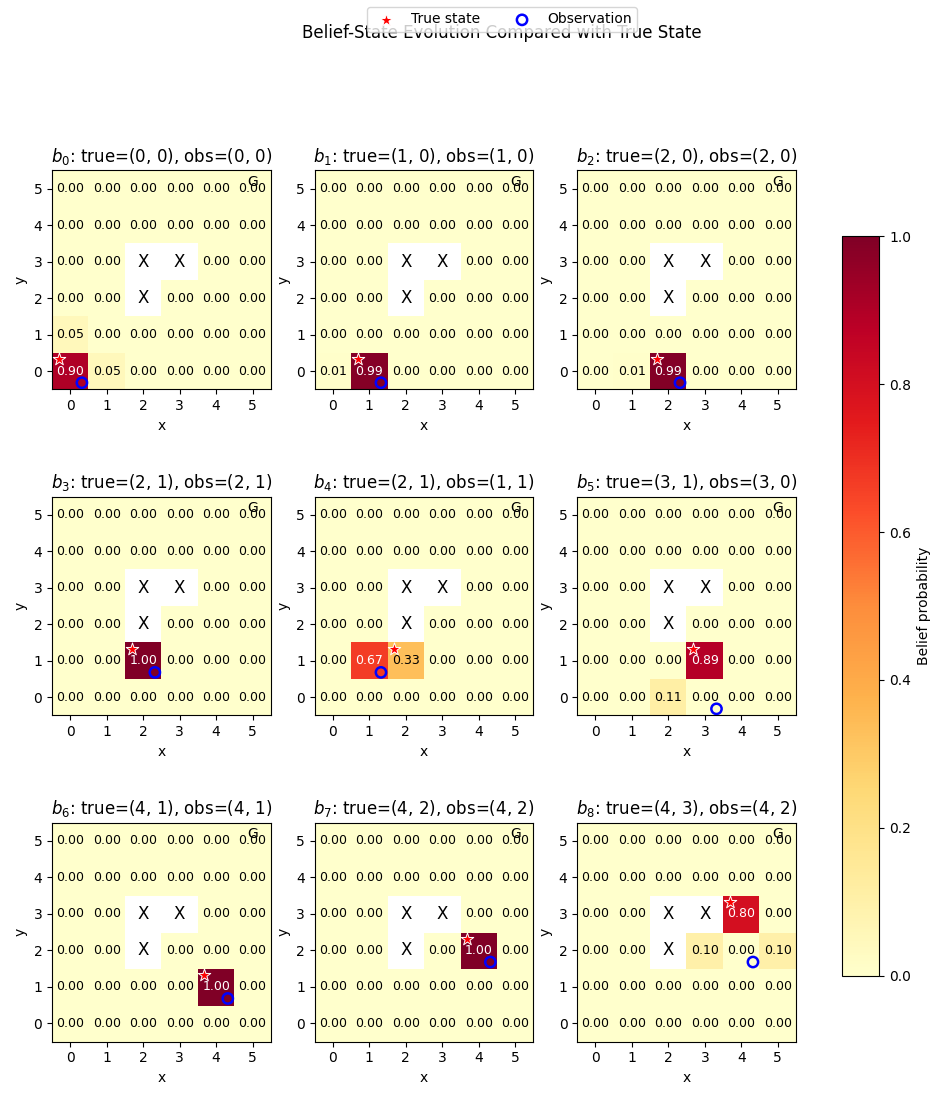
\includegraphics[height=5.95in,width=\textwidth,keepaspectratio]{report_figures/2b.png}
\end{center}

\clearpage
\subsection{3}
\texttt{MAP.py}
\begin{lstlisting}[numbers=none]
best_action = np.argmin([stage_cost_c(most_likely_state, a) + sum([transition_prob[a, most_likely_state, s_next] * J_opt[t + 1, s_next] for s_next in range(S)]) for a in range(A)])
\end{lstlisting}

\subsection{4}
The QMDP policy uses the entire belief distribution rather than only the most likely state. For each action, it computes the expected MDP cost by weighting the cost associated with each possible current state by its belief probability, and then chooses the action with the smallest expected cost. Intuitively, it accounts for uncertainty in the robot’s location instead of committing to a single estimated state.


\subsection{5}
\input{q2_5.tex}
